	% Copyright 2004 by Till Tantau <tantau@users.sourceforge.net>.
%
% In principle, this file can be redistributed and/or modified under
% the terms of the GNU Public License, version 2.
%
% However, this file is supposed to be a template to be modified
% for your own needs. For this reason, if you use this file as a
% template and not specifically distribute it as part of a another
% package/program, I grant the extra permission to freely copy and
% modify this file as you see fit and even to delete this copyright
% notice. 

\documentclass{beamer}

% There are many different themes available for Beamer. A comprehensive
% list with examples is given here:
% http://deic.uab.es/~iblanes/beamer_gallery/index_by_theme.html
% You can uncomment the themes below if you would like to use a different
% one:
%\usetheme{AnnArbor}
%\usetheme{Antibes}
%\usetheme{Bergen}
%\usetheme{Berkeley}
%\usetheme{Berlin}
%\usetheme{Boadilla}
%\usetheme{boxes}
%\usetheme{CambridgeUS}
%\usetheme{Copenhagen}
%\usetheme{Darmstadt}
%\usetheme{default}
%\usetheme{Frankfurt}
%\usetheme{Goettingen}
%\usetheme{Hannover}
%\usetheme{Ilmenau}
%\usetheme{JuanLesPins}
%\usetheme{Luebeck}
\usetheme{Madrid}
%\usetheme{Malmoe}
%\usetheme{Marburg}
%\usetheme{Montpellier}
%\usetheme{PaloAlto}
%\usetheme{Pittsburgh}
%\usetheme{Rochester}
%\usetheme{Singapore}
%\usetheme{Szeged}
%\usetheme{Warsaw}

\usepackage{media9}
\usepackage{ragged2e}
\usepackage{tikz}
\usepackage{epstopdf}
\usepackage{algorithm2e}
%from videos tutorial
\usepackage[utf8]{inputenc}
\usepackage[T1]{fontenc}
\usepackage{parskip}

\usepackage{graphicx}
\usepackage{media9}
%\usepackage{algorithm}

% Customize Warsaw color 
\setbeamercolor*{palette primary}{use=structure,fg=white,bg=red!50!black}
\setbeamercolor*{palette secondary}{use=structure,fg=white,bg=red!60!black}
\setbeamercolor*{palette tertiary}{use=structure,fg=white,bg=red!70!black}
\part{First Presentation}
% Customize Warsaw block title and background colors
\setbeamertemplate{section in toc}[ball unnumbered]
\setbeamercolor{block title}{bg=red!50!black,fg=white}

\title{Research Summary}


% % A subtitle is optional and this may be deleted
\subtitle{Prospective Ph.D. Student at Carnegie Mellon University}

\author[A.Elhussein]{Amr~Elhussein  \\\and
Advisor: Dr. Suruz Miah}
% - Give the names in the same order as the appear in the paper.
% - Use the \inst{?} command only if the authors have different
%   affiliation.

\institute[Bradley University] % (optional, but mostly needed)
{
  Department of Electrical and Computer Engineering\\
  Bradley University\\
  1501 W. Bradley Avenue\\
  Peoria, IL, 61625, USA
}
% - Use the \inst command only if there are several affiliations.
% - Keep it simple, no one is interested in your street address.

\date[February~8,~2021]{Monday, February~8,~2021}
% - Either use conference name or its abbreviation.
% - Not really informative to the audience, more for people (including
%   yourself) who are reading the slides online

\logo{\hfill\href{http://www.bradley.edu}{
\includegraphics[width=0.75cm]{figs/logoBU1-Print}}}  % place logo in every page 


\subject{Mobile Robot Localization}
% This is only inserted into the PDF information catalog. Can be left
% out. 

% If you have a file called "university-logo-filename.xxx", where xxx
% is a graphic format that can be processed by latex or pdflatex,
% resp., then you can add a logo as follows:

% \pgfdeclareimage[height=0.5cm]{university-logo}{university-logo-filename}
% \logo{\pgfuseimage{university-logo}}

% Delete this, if you do not want the table of contents to pop up at
% the beginning of each subsection:
%\AtBeginSubsection[]
%{
 % \begin{frame}<beamer>{Outline}
  %  \tableofcontents[currentsection,currentsubsection]
  %\end{frame}
%}

% Let's get started
\begin{document}

\begin{frame}
  \titlepage
\end{frame}

\begin{frame}{Outline}
  \tableofcontents
  % You might wish to add the option [pausesections]
\end{frame}

% Section and subsections will appear in the presentation overview
% and table of contents.

\section{Concept of Area Coverage Algorithm}
\begin{frame}{Area Coverage Algorithm}
\begin{columns}
\begin{column}{0.5\textwidth}
\begin{center}
\begin{figure}
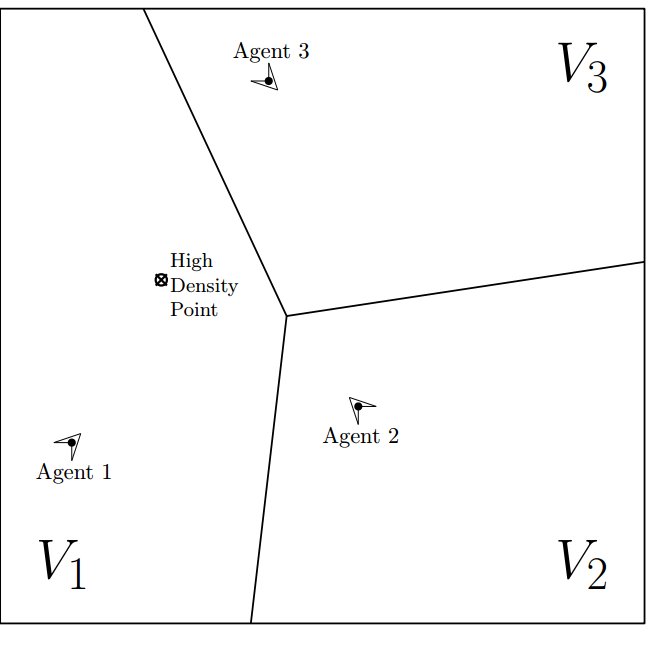
\includegraphics[scale=0.2]{figs/img/voroni.png}
\caption{Voroni regions}
\end{figure}
\end{center}
\end{column}
\begin{column}{0.5\textwidth}
\begin{center}
\begin{figure}
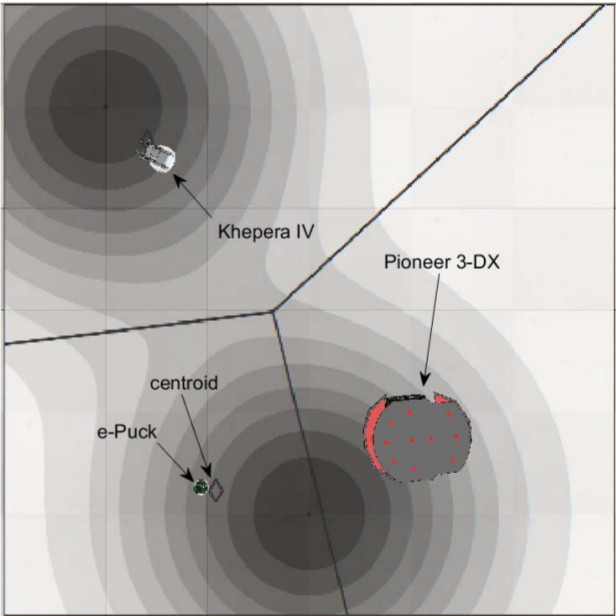
\includegraphics[scale=0.2]{figs/img/areaCoverage.png}
\caption{V-rep simulation}
\end{figure}
\end{center}
\end{column}
\end{columns}
\end{frame}
%--------------------
\section{Reinforcment learning}
\begin{frame}{Problem Setup}

\begin{figure}
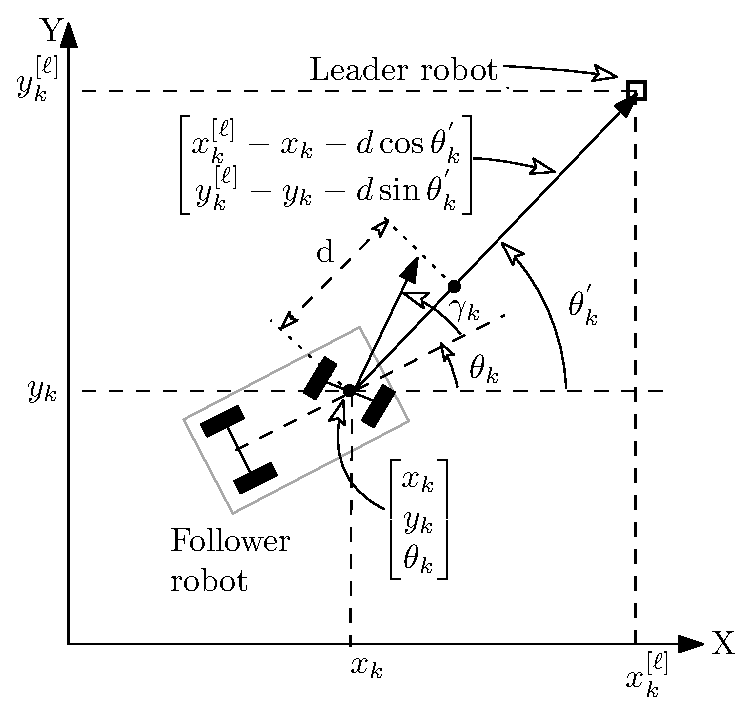
\includegraphics[scale=0.5]{figs/ipe/LF-Setup.eps}
\caption{Problem Setup}
\end{figure}

\end{frame}

%--------------------------------
\section{Equations}
\begin{frame}{Equations}
\begin{equation}
{\bf u}_k=[\nu_k,\gamma_k]^T\in\mathbb{R}^2
\end{equation}

\begin{equation}
{e}_k^T = 
\begin{bmatrix}
x_k^{[\ell]} - x_k - d\cos\theta_k^{'},
y_k^{[\ell]} - y_k - d\sin\theta_k^{'},
\theta_k^{'} - \theta_k
\end{bmatrix}
\end{equation}
\begin{equation}
V({\bf e}_k,{\bf u}_k) = \sum_{\kappa=k}^\infty \frac{1}{2}\left({\bf e}_\kappa^T\, {\bf Q}\, {\bf e}_\kappa + {\bf u}_\kappa^T \, {\bf R}\, {\bf u_\kappa}\right)
\end{equation}
\begin{equation}
\mathbf{z}_k = \left[\mathbf{e}_k ,\mathbf{u}_k\right]^T\in\mathbb{R}^5
\end{equation}
\begin{equation}
\hat{V}(\mathbf{z}_k) = \frac{1}{2}\mathbf{z}_k^T\, {\mathbf{P}}\, \mathbf{z}_k + \hat{V}(\mathbf{z}_{k+1}),
\end{equation}
\end{frame}
%------------
\section{Neural Network}
\begin{frame}
\begin{figure}
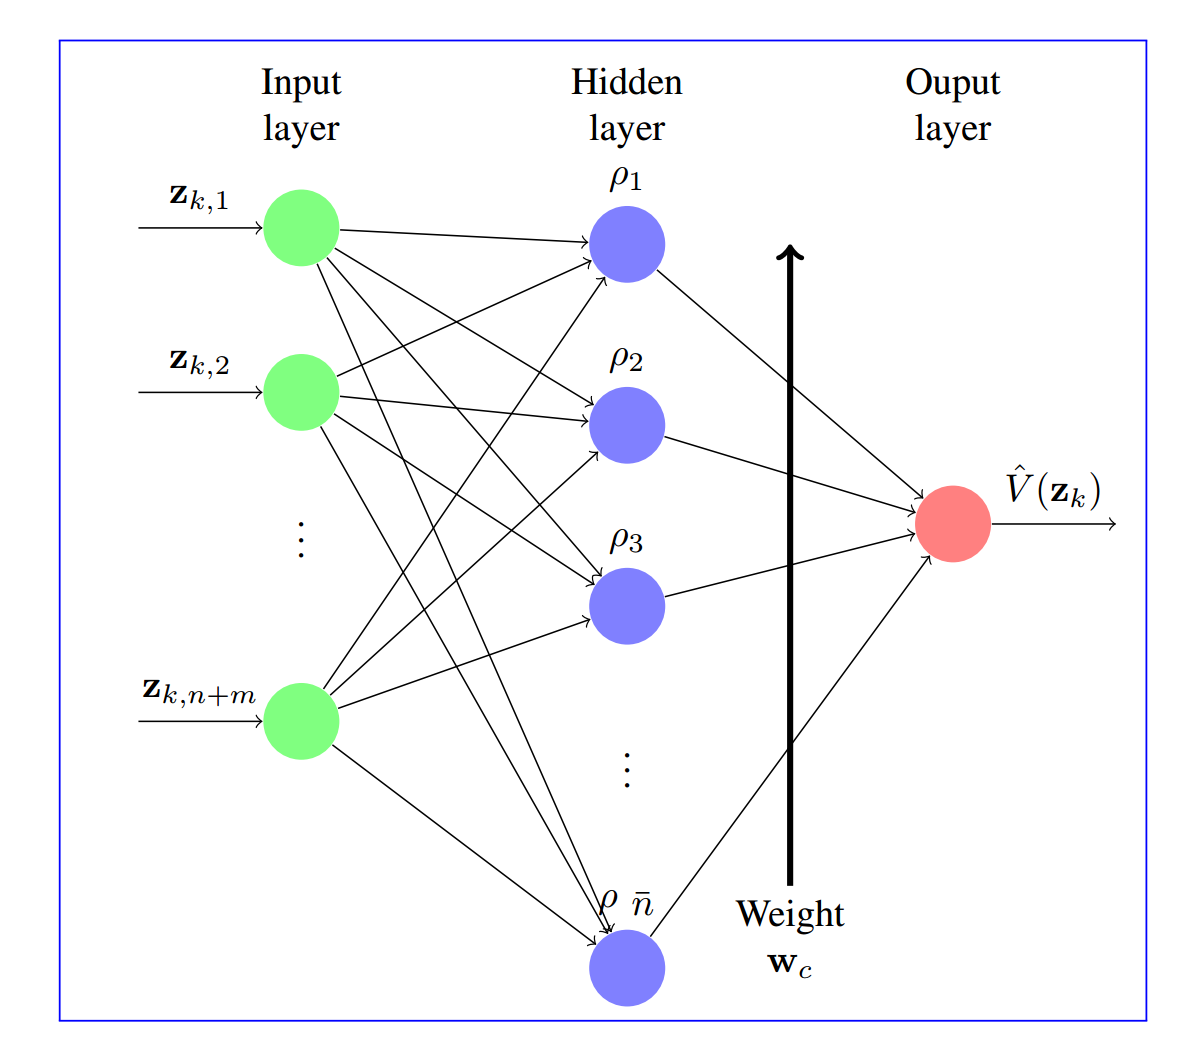
\includegraphics[scale=0.2]{figs/img/criticNeuralNetwork.png}
\caption{Neural Network Architecture}
\end{figure}
\end{frame}
\section{Milestones}
\begin{frame}{Milestones}
\begin{block}{Milestones}
\begin{itemize}
\item Merge the leader follower model free reinforcment learning as a function in the area coverage algorithm.
\item Simulate the results in matlab.
\item Integrate matlab with CoppeliaSim and perform the simulation.  
\end{itemize}
\end{block}
\end{frame}
%----------------------------------
\section*{Questions}
\begin{frame}
\begin{LARGE}
\begin{center}
Questions?
\end{center}
\end{LARGE}
\end{frame}
%-----------------------
\end{document}








	